\documentclass[tikz, border=10pt]{standalone}
\usepackage{amsmath}
\usepackage{tikz}
\usetikzlibrary{decorations.pathmorphing, arrows.meta, calc, backgrounds}

\definecolor{navybg}{RGB}{13,27,42}
\definecolor{source1col}{RGB}{0,220,255}
\definecolor{source2col}{RGB}{255,165,0}
\definecolor{photoncol}{RGB}{255,215,0}
\definecolor{starglow}{RGB}{255,255,200}
\definecolor{labelcol}{RGB}{220,220,220}
\definecolor{plotbg}{RGB}{25,40,60}

\begin{document}
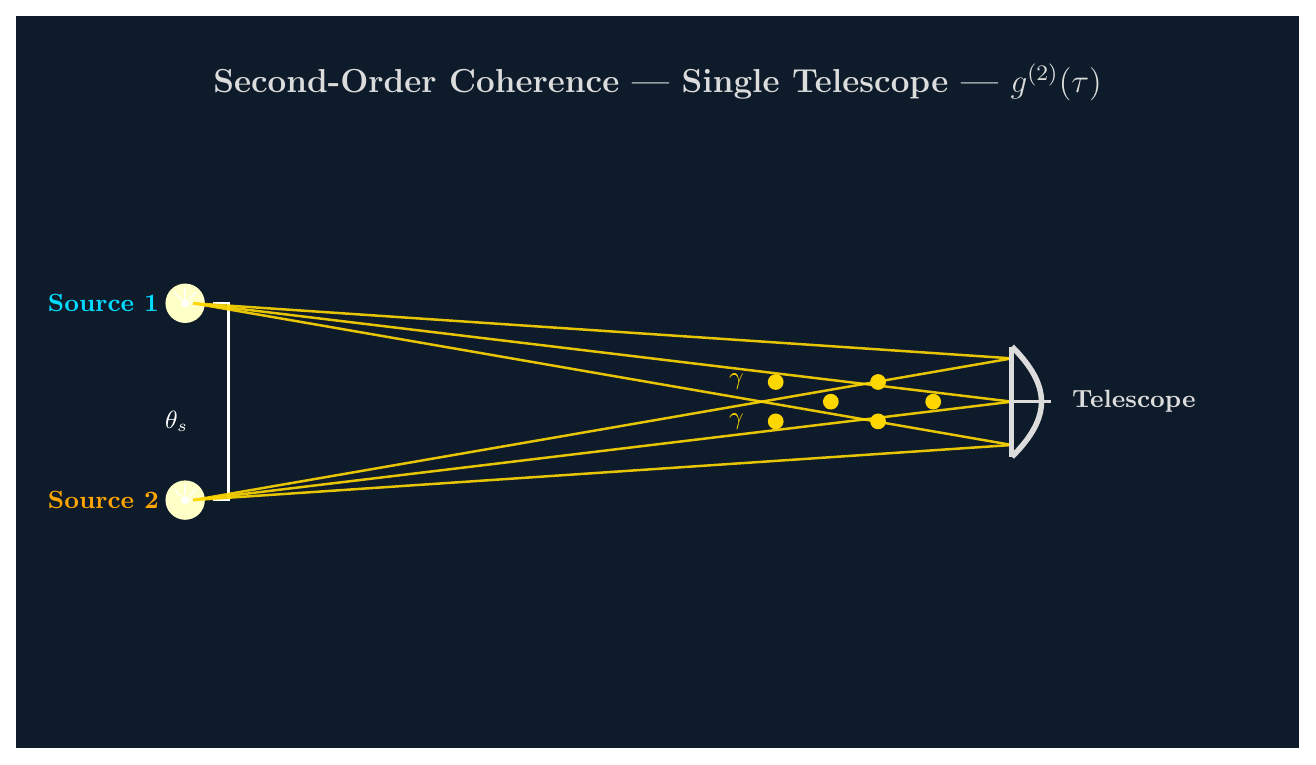
\begin{tikzpicture}[
    background rectangle/.style={fill=navybg},
    show background rectangle,
    arr/.style={-{Stealth[length=6pt]}, line width=1.2pt},
    arrthin/.style={-{Stealth[length=4pt]}, line width=0.8pt},
    mybox/.style={draw=labelcol, fill=plotbg, rounded corners=4pt,
                  line width=1pt, text=labelcol, font=\small,
                  inner sep=5pt, align=center},
]

\path[use as bounding box] (0,0) rectangle (16,9);

% ════════════════════════════════════════════════════════
% 0. TITLE
% ════════════════════════════════════════════════════════
\node[text=labelcol, font=\large\bfseries] at (8.0, 8.3)
    {Second-Order Coherence \textemdash\ Single Telescope
     \textemdash\ $g^{(2)}(\tau)$};

% ════════════════════════════════════════════════════════
% 1. TWO POINT SOURCES (LEFT SIDE)
% ════════════════════════════════════════════════════════
\coordinate (S1) at (2.0, 5.5);
\coordinate (S2) at (2.0, 3.0);

% Glow halos S1
\foreach \r/\op in {0.25/15, 0.15/30, 0.08/60}{
    \fill[starglow, opacity=\op] (S1) circle (\r);
}
\fill[white] (S1) circle (0.05);
\foreach \ang in {0,45,90,135}{
    \draw[white, line width=0.6pt, opacity=0.8]
        ($(S1)+(\ang:0.06)$) -- ($(S1)+(\ang:0.20)$);
}
\node[text=source1col, font=\small\bfseries, left=6pt] at (S1) {Source 1};

% Glow halos S2
\foreach \r/\op in {0.25/15, 0.15/30, 0.08/60}{
    \fill[starglow, opacity=\op] (S2) circle (\r);
}
\fill[white] (S2) circle (0.05);
\foreach \ang in {0,45,90,135}{
    \draw[white, line width=0.6pt, opacity=0.8]
        ($(S2)+(\ang:0.06)$) -- ($(S2)+(\ang:0.20)$);
}
\node[text=source2col, font=\small\bfseries, left=6pt] at (S2) {Source 2};

% Angular separation brace
\draw[white, line width=0.8pt]
    ($(S1)+(0.35, 0)$) -- ($(S1)+(0.55, 0)$)
    -- ($(S2)+(0.55, 0)$) -- ($(S2)+(0.35, 0)$);
\node[text=white, font=\small, right=2pt] at (1.55, 4.0) {$\theta_s$};

% ════════════════════════════════════════════════════════
% 2. PHOTON BULLETS NEAR TELESCOPE
% ════════════════════════════════════════════════════════
\coordinate (TEL) at (12.5, 4.25);

% Solid lines from S1 to telescope aperture
\draw[photoncol, line width=0.9pt, opacity=0.9]
    ($(S1)+(0.1, 0)$) -- ($(TEL)+(0.0, 0.55)$);
\draw[photoncol, line width=0.9pt, opacity=0.9]
    ($(S1)+(0.1, 0)$) -- ($(TEL)+(0.0, 0.0)$);
\draw[photoncol, line width=0.9pt, opacity=0.9]
    ($(S1)+(0.1, 0)$) -- ($(TEL)+(0.0,-0.55)$);

% Solid lines from S2 to telescope aperture
\draw[photoncol, line width=0.9pt, opacity=0.9]
    ($(S2)+(0.1, 0)$) -- ($(TEL)+(0.0, 0.55)$);
\draw[photoncol, line width=0.9pt, opacity=0.9]
    ($(S2)+(0.1, 0)$) -- ($(TEL)+(0.0, 0.0)$);
\draw[photoncol, line width=0.9pt, opacity=0.9]
    ($(S2)+(0.1, 0)$) -- ($(TEL)+(0.0,-0.55)$);

% Photon bullets close to telescope — from S1 direction
\fill[photoncol] (9.5, 4.5) circle (0.10);
\fill[photoncol] (10.2, 4.25) circle (0.10);
\fill[photoncol] (9.5, 4.0) circle (0.10);

% Photon bullets close to telescope — from S2 direction
\fill[photoncol] (10.8, 4.5) circle (0.10);
\fill[photoncol] (11.5, 4.25) circle (0.10);
\fill[photoncol] (10.8, 4.0) circle (0.10);

% h-nu labels on select bullets
\node[text=photoncol, font=\small] at (9.0, 4.5) {$\gamma$};
\node[text=photoncol, font=\small] at (9.0, 4.0) {$\gamma$};

% ════════════════════════════════════════════════════════
% 3. TELESCOPE (RIGHT SIDE, facing left)
% ════════════════════════════════════════════════════════
\draw[labelcol, line width=2pt]
    ($(TEL)+(0.0,  0.7)$)
    .. controls ($(TEL)+(0.5, 0.2)$) and ($(TEL)+(0.5,-0.2)$) ..
    ($(TEL)+(0.0, -0.7)$);
\draw[labelcol, line width=1.8pt]
    ($(TEL)+(0.0, 0.7)$) -- ($(TEL)+(0.0,-0.7)$);
\draw[labelcol, line width=1.0pt]
    ($(TEL)+(0.0, 0.0)$) -- ($(TEL)+(0.5, 0.0)$);

\node[text=labelcol, font=\small\bfseries, right=4pt]
    at ($(TEL)+(0.5, 0.0)$) {Telescope};

\end{tikzpicture}
\end{document}
